\documentclass{beamer}
\usepackage[T1]{fontenc}
\usepackage[utf8]{inputenc}

\usetheme{Madrid}
\usecolortheme{default}
\usepackage{amsmath,amssymb,amsfonts,amsthm}
\usepackage{mathtools}
\usepackage{txfonts}
\usepackage{tkz-euclide}
\usepackage{listings}
\usepackage{adjustbox}
\usepackage{array}
\usepackage{gensymb}
\usepackage{tabularx}
\usepackage{gvv}
\usepackage{lmodern}
\usepackage{circuitikz}
\usepackage{tikz}
\lstset{literate={·}{{$\cdot$}}1 {λ}{{$\lambda$}}1 {→}{{$\to$}}1}
\usepackage{graphicx}

\setbeamertemplate{page number in head/foot}[totalframenumber]

\usepackage{tcolorbox}
\tcbuselibrary{minted,breakable,xparse,skins}



\definecolor{bg}{gray}{0.95}
\DeclareTCBListing{mintedbox}{O{}m!O{}}{%
  breakable=true,
  listing engine=minted,
  listing only,
  minted language=#2,
  minted style=default,
  minted options={%
    linenos,
    gobble=0,
    breaklines=true,
    breakafter=,,
    fontsize=\small,
    numbersep=8pt,
    #1},
  boxsep=0pt,
  left skip=0pt,
  right skip=0pt,
  left=25pt,
  right=0pt,
  top=3pt,
  bottom=3pt,
  arc=5pt,
  leftrule=0pt,
  rightrule=0pt,
  bottomrule=2pt,
  toprule=2pt,
  colback=bg,
  colframe=orange!70,
  enhanced,
  overlay={%
    \begin{tcbclipinterior}
    \fill[orange!20!white] (frame.south west) rectangle ([xshift=20pt]frame.north west);
    \end{tcbclipinterior}},
  #3,
}
\lstset{
    language=C,
    basicstyle=\ttfamily\small,
    keywordstyle=\color{blue},
    stringstyle=\color{orange},
    commentstyle=\color{green!60!black},
    numbers=left,
    numberstyle=\tiny\color{gray},
    breaklines=true,
    showstringspaces=false,
}
\title{5.8.8}
\subtitle{Application problem}
\author{EE25BTECH11010 - Arsh Dhoke}
\date{}
\begin{document}


\begin{frame}
  \titlepage
\end{frame}
\begin{frame}{Question}
Places A and B are 100km apart on a highway. One car starts from A and another from B at the same time. 
If the cars travel in the same direction at different speeds, they meet in 5 hrs. 
If they travel towards each other, they meet in 1 hr. 
Find the speeds of the two cars.
\end{frame}

\begin{frame}{Solution: Step 1}
Cars meet in 1 hr when moving towards each other:
\begin{align}
v_1 + v_2 &= \frac{100}{1} = 100
\end{align}

Cars meet in 5 hr when moving in the same direction:
\begin{align}
v_1 - v_2 &= \frac{100}{5} = 20
\end{align}
\end{frame}

\begin{frame}{Solution: Vector Form}
The equations can be expressed as
\begin{align}
\myvec{1 & 1}\myvec{v_1 \\ v_2} &= 100, \\
\myvec{1 & -1}\myvec{v_1 \\ v_2} &= 20.
\end{align}

Let 
\begin{align}
\vec{r_1} = \myvec{1 & 1}, \quad \vec{r_2} = \myvec{1 & -1}.
\end{align}
Then $\vec{r_1} \cdot \vec{r_2} = 0$, showing that the two rows are orthogonal.
\end{frame}

\begin{frame}{Solution: Using Orthogonality}
Let
\begin{align}
\myvec{v_1 \\ v_2} = c_1\,\vec{r_1}^{T} + c_2\,\vec{r_2}^{T}.
\end{align}

Taking dot products with $\vec{r_1}$ and $\vec{r_2}$,
\begin{align}
\vec{r_1}\cdot\myvec{v_1 \\ v_2} &= c_1\,\vec{r_1}\cdot\vec{r_1} = 100, \\
\vec{r_2}\cdot\myvec{v_1 \\ v_2} &= c_2\,\vec{r_2}\cdot\vec{r_2} = 20.
\end{align}
\end{frame}

\begin{frame}{Solution: Compute Coefficients}
Since $\|\vec{r_1}\|^2 = \|\vec{r_2}\|^2 = 2$,
\begin{align}
c_1 = \frac{100}{2} = 50, \quad c_2 = \frac{20}{2} = 10.
\end{align}

Therefore,
\begin{align}
\myvec{v_1 \\ v_2} &= 50\,\vec{r_1}^{T} + 10\,\vec{r_2}^{T} \\
&= 50\myvec{1 \\ 1} + 10\myvec{1 \\ -1} \\
&= \myvec{60 \\ 40}.
\end{align}
\end{frame}

\begin{frame}{Final Answer}
\begin{align}
\boxed{v_1 = 60~\text{km/h}}, \quad \boxed{v_2 = 40~\text{km/h}}
\end{align}
\end{frame}

\begin{frame}{Graphical Representation}
\begin{figure}[ht!]
\centering
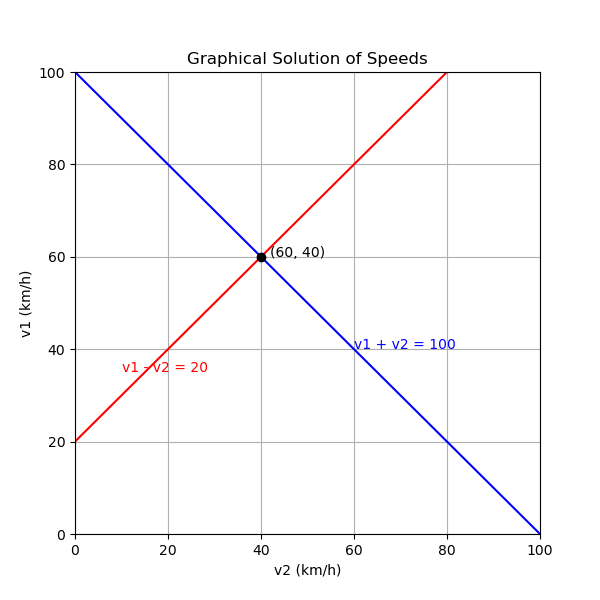
\includegraphics[height=0.6\textheight, keepaspectratio]{figs/speed.png}
\caption{Graphical solution of speeds}
\end{figure}
\end{frame}

\begin{frame}[fragile]
    \frametitle{C Code}
\begin{lstlisting}
#include <stdio.h>

void solve_car_speeds(double distance, double time_same_dir, double time_towards, double *v1, double *v2) {
    double sum_speeds = distance / time_towards;
    double diff_speeds = distance / time_same_dir;

    *v1 = (sum_speeds + diff_speeds) / 2.0;
    *v2 = sum_speeds - *v1;
}

\end{lstlisting}
\end{frame}

\begin{frame}[fragile]
    \frametitle{Python Code}
\begin{lstlisting}
import matplotlib.pyplot as plt
import numpy as np

# Define v2 range
v2 = np.linspace(0, 100, 200)

# Equations
v1_towards = 100 - v2      # v1 + v2 = 100
v1_same = 20 + v2          # v1 - v2 = 20

# Plot
plt.figure(figsize=(6,6))
plt.plot(v2, v1_towards, color='blue')
plt.plot(v2, v1_same, color='red')

# Intersection point
v2_meet = 40
v1_meet = 60
\end{lstlisting}
\end{frame}

\begin{frame}[fragile]
    \frametitle{Python Code}
\begin{lstlisting}
plt.plot(v2_meet, v1_meet, 'ko')  # solution point

# Annotate the lines
plt.text(60, 40, 'v1 + v2 = 100', color='blue')
plt.text(10, 35, 'v1 - v2 = 20', color='red')

# Annotate solution point
plt.text(v2_meet + 2, v1_meet, '(60, 40)', color='black')

plt.xlabel('v2 (km/h)')
plt.ylabel('v1 (km/h)')
plt.title('Graphical Solution of Speeds')
plt.xlim(0, 100)
plt.ylim(0, 100)
plt.grid(True)
plt.savefig("/home/arsh-dhoke/ee1030-2025/ee25btech11010/matgeo/5.8.8/figs/speed.png")
plt.show()

\end{lstlisting}
\end{frame}

\begin{frame}[fragile]
    \frametitle{Python+ C Code}
\begin{lstlisting}
import ctypes
import numpy as np
import matplotlib.pyplot as plt

# Load the shared library
lib = ctypes.CDLL('./code.so')

# Define argument and return types
lib.solve_car_speeds.argtypes = [
    ctypes.c_double, ctypes.c_double, ctypes.c_double,
    ctypes.POINTER(ctypes.c_double), ctypes.POINTER(ctypes.c_double)
]

# Function to call C function
def get_speeds(distance, time_same_dir, time_towards):
    v1 = ctypes.c_double()
    v2 = ctypes.c_double()
    \end{lstlisting}
\end{frame}

\begin{frame}[fragile]
    \frametitle{Python+ C Code}
\begin{lstlisting}
    lib.solve_car_speeds(distance, time_same_dir, time_towards, ctypes.byref(v1), ctypes.byref(v2))
    return v1.value, v2.value

# Example
distance = 100.0
time_same_dir = 5.0
time_towards = 1.0

v1, v2 = get_speeds(distance, time_same_dir, time_towards)
print(f"v1 = {v1}, v2 = {v2}")

# Plot the lines v1 + v2 = distance / time_towards and v1 - v2 = distance / time_same_dir
v2_vals = np.linspace(0, 100, 200)
v1_towards = distance / time_towards - v2_vals
v1_same = distance / time_same_dir + v2_vals
\end{lstlisting}
\end{frame}

\begin{frame}[fragile]
    \frametitle{Python+ C Code}
\begin{lstlisting}
plt.plot(v2_vals, v1_towards, color='blue')
plt.plot(v2_vals, v1_same, color='red')
plt.plot(v2, v1, 'ko')  # intersection
plt.xlabel('v2 (km/h)')
plt.ylabel('v1 (km/h)')
plt.grid(True)
plt.savefig("/home/arsh-dhoke/ee1030-2025/ee25btech11010/matgeo/5.8.8/figs/speed.png")
plt.show()

\end{lstlisting}
\end{frame}
\end{document}

